\ylDisplay{Tiik} % Ülesande nimi
{Taavi Pungas} % Autor
{lõppvoor} % Voor
{2013} % Aasta
{G 6} % Ülesande nr.
{5} % Raskustase
{
% Teema: Varia
\ifStatement
\begin{wrapfigure}{r}{0.25\textwidth}%
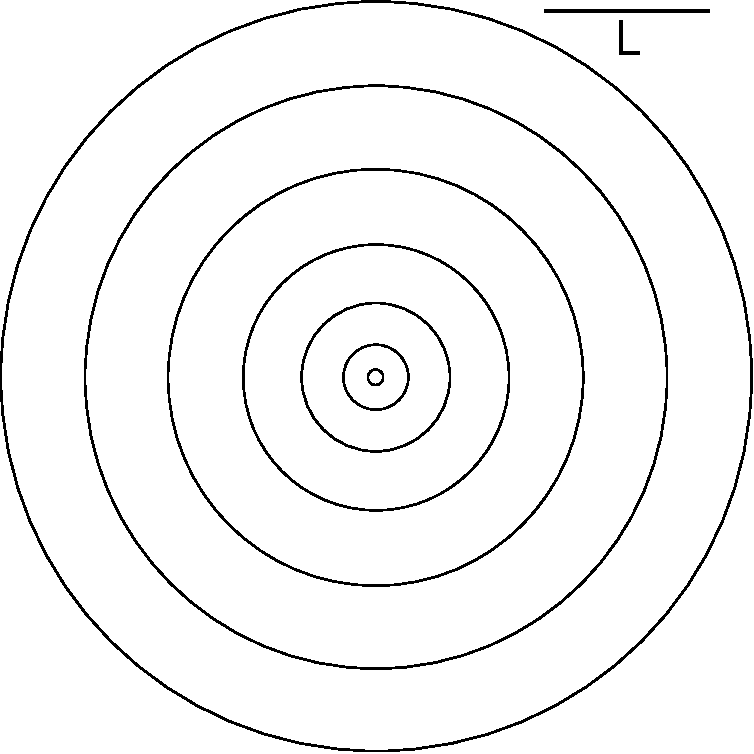
\includegraphics[width=\linewidth]{2013-v3g-06-lained}%
\end{wrapfigure}
Vaatleme tiiki visatud kivi ümber tekkinud lainetust. Kui kivi kukub vette,
tekib suur hulk erinevate lainepikkustega häiritusi, millest igaüks levib
omaette kiirusega. Nende liitumisel moodustub lainehari, mille liikumist
saame vaadelda. Joonisele (suuremalt lisalehele) on iga kindla ajavahemiku järel kantud selle
laineharja asukoht, mõõtkavaks sirglõik pikkusega~$L$. Laineharja kiirus $v$
sõltub seda parasjagu moodustavate komponentide lainepikkustest $\lambda$ ja vee
sügavusest $h$. Kui kivi vettekukkumisest möödunud aeg $t$ on väike, siis
koosneb lainehari lainepikkustest $\lambda \ll h$ ning laineharja kiirus sõltub
ajast seose $v \approx \frac{gt}{\pi}$ järgi. Kaugemal, kus laineharja
moodustavad häiritused lainepikkusega $\lambda \gg h$, liigub see kiirusega $v
\approx \sqrt{hg}$. Hinnake sügavust $h$ eeldusel, et see oli terve tiigi
ulatuses sama. Vastus andke suhtena~$h/L$.
\fi


\ifHint
Jooniselt on võimalik mõõta ringide läbimõõdud. Kasutades lühikese lainepikkusega lainete kiiruse valemit, on esimeste ringide raadiuste põhjal võimalik arvutada kulunud ajavahemikud.
\fi


\ifSolution
Mõõdame jooniselt ringide läbimõõdud, saame 0,1; 0,4; 0,9; 1,6; 2,5; 3,5 ja 4,5 ühikut $L$-i. Näeme, et alguses on liikumine ühtlaselt kiirenev ehk kehtib $\lambda \ll h$ seos $r \approx \frac{gt^2}{2 \pi}$. Sellest saame arvutada esimestele ringidele vastavad ajahetked, $t = \sqrt{\frac{2 \pi r}{g}}$: $\sqrt{\frac{\pi L}{10 g}}$, $2 \sqrt{\frac{\pi L}{10 g}}$, $3 \sqrt{\frac{\pi L}{10 g}}$, $4 \sqrt{\frac{\pi L}{10 g}}$, $5 \sqrt{\frac{\pi L}{10 g}}$. Näeme, et joonise tegemiseks kasutatud ajavahemik oli $T=\sqrt{\frac{\pi L}{10 g}}$.
Hiljem on liikumine ühtlane, kiirusega $v=\frac{L}{T}=\sqrt{\frac{10 L g}{\pi}}$. Teisalt teame, et $v \approx \sqrt{hg}$, seega tiigi sügavus on $h \approx \frac{v^2}{g} = \frac{10 L}{\pi}$. Vastus: $h/L = \frac{10}{\pi} \approx \SI{3,2}{}$.
\fi


\ifEngStatement
% Problem name: Pond
\begin{wrapfigure}{r}{0.25\textwidth}%
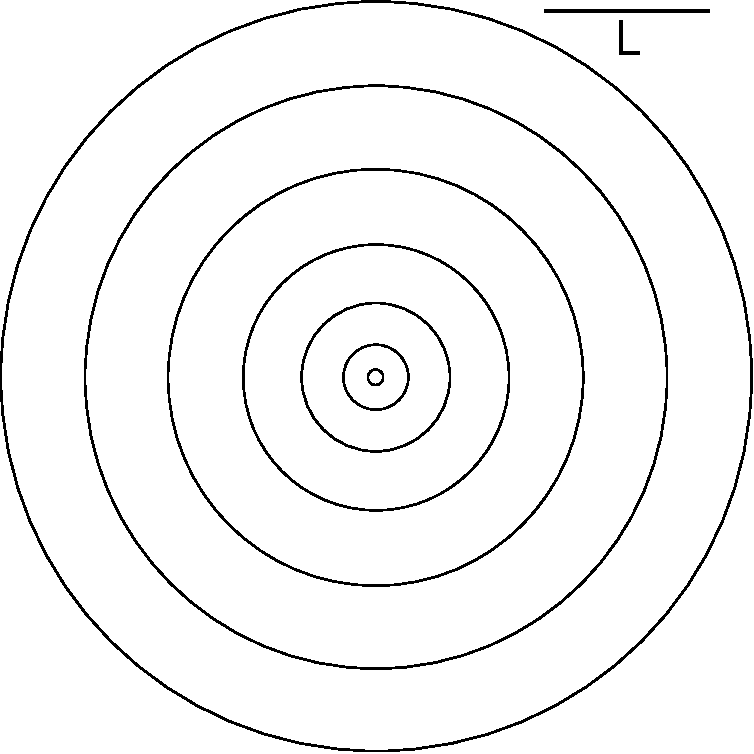
\includegraphics[width=\linewidth]{2013-v3g-06-lained}%
\end{wrapfigure}
Let us take a look at the waves forming around a stone thrown into a pond. When the stone falls into the water a big amount of disturbances with different wavelengths form, each of them propagating with their own speed. When they are merged a wave crest is formed and we can observe the crest’s movement. The locations of this crest, each of them after a specific amount of time, are shown in the figure, the scale is a straight line of length $L$. The speed $v$ of the crest depends on the wavelengths $\lambda$ of the components it is currently made of and on the depth $h$ of the water. If a time $t$ that has passed from throwing the stone into the water is small then the crest consists of wavelengths $\lambda \ll h$ and the speed of the wavelength depends on the time as $v \approx \frac{gt}{\pi}$. Further, where the disturbances that create a crest have a wavelength $\lambda \gg h$, the wavelength moves with a speed $v
\approx \sqrt{hg}$. Evaluate the depth $h$ assuming that it is the same over the whole pond. Give the answer as a ratio of $h/L$.
\fi


\ifEngHint
From the figure you can measure the diameters of the circles. Using the speed equation for waves with small wavelength you can calculate the time periods covered based on the radiuses of the first circles.
\fi


\ifEngSolution
Let us measure the diameters of the circles in the figure, we get 0.1; 0.4; 0.9; 1.6; 2.5; 3.5 and 4.5 units of $L$. We see that initially the movement is evenly accelerating meaning that the relation $r \approx \frac{gt^2}{2 \pi}$ applies $\lambda \ll h$. From this we can calculate the moments of time corresponding to the first circles $t = \sqrt{\frac{2 \pi r}{g}}$: $\sqrt{\frac{\pi L}{10 g}}$, $2 \sqrt{\frac{\pi L}{10 g}}$, $3 \sqrt{\frac{\pi L}{10 g}}$, $4 \sqrt{\frac{\pi L}{10 g}}$, $5 \sqrt{\frac{\pi L}{10 g}}$. We see that the time period used in the making of figure was $T=\sqrt{\frac{\pi L}{10 g}}$. Later the movement is uniform, with a speed $v=\frac{L}{T}=\sqrt{\frac{10 L g}{\pi}}$. On the other hand we know that $v \approx \sqrt{hg}$, therefore the pond's depth is $h \approx \frac{v^2}{g} = \frac{10 L}{\pi}$. The answer: $h/L = \frac{10}{\pi} \approx \SI{3,2}{}$
\fi
}